\documentclass[10pt,journal]{IEEEtran}

% Use the postscript times font!
\usepackage{times}
\usepackage{soul}
\usepackage{url}
\usepackage[hidelinks]{hyperref}
\usepackage[utf8, utf8x]{inputenc}
\usepackage[small]{caption}
\usepackage{graphicx}
\usepackage{amsmath}
\usepackage{booktabs}
\usepackage{algorithm}
\usepackage{algorithmic}
\usepackage{subcaption}
\urlstyle{same}

\usepackage{tikz}
\usepackage{xargs}
\usepackage{menukeys}
\usepackage[colorinlistoftodos,prependcaption,textsize=tiny]{todonotes}
\newcommandx{\unsure}[2][1=]{\todo[linecolor=red,backgroundcolor=red!25,bordercolor=red,#1]{#2}}
\newcommandx{\change}[2][1=]{\todo[linecolor=blue,backgroundcolor=blue!25,bordercolor=blue,#1]{#2}}
\newcommandx{\info}[2][1=]{\todo[linecolor=green,backgroundcolor=green!25,bordercolor=green,#1]{#2}}
\newcommandx{\improvement}[2][1=]{\todo[linecolor=purple,backgroundcolor=purple!25,bordercolor=purple,#1]{#2}}
\newcommandx{\thiswillnotshow}[2][1=]{\todo[disable,#1]{#2}}

\usepackage{amsmath}
\usepackage{amssymb}
\newcommand{\R}{\mathbb{R}}
\newcommand{\D}{\mathbb{D}}

\title{IOMeans: Classifying Multi-concurrent I/O threads using Spatio-Tempo Mapping}

\begin{document}

\maketitle

\listoftodos[TODO]

\todo{use word template}

\section{Introduction}

Because secondary storage is physically farthest away from CPU in modern memory hierarchy
and shared by many concurrent processes,
I/O accesses bear less locality and is more complexity than that of memory workloads~\cite{yang1992novel}.
Much research has been done to employ prefetch as one weapon to bridge the speed gap between memory and storage.
However, storage side prefetching mainly optimized for relatively simple I/O patterns.
DiskSeen~\cite{ding2007diskseen} adopts sequential prefetching for disk I/O.
Competitive prefetching~\cite{li2007competitive} optimizes the sequential prefetching for multiple concurrent I/O stream.
In order to optimize the workloads that are not sequential,
Chen et. al.~\cite{chen2008hiding} perform pre-execution and keep a record of the request for prefetching.
Signature-based parallel prefetching~\cite{byna2008parallel} calculates the signature of request sequence to match future request sequence. %signature-based prefetching.
Lots of researchers develop solutions to learn patterns for
specific workloads that are characterized by stable and repeatable patterns.
For example, Anwar et. al.~\cite{anwar2018improving} seek to perform
prefetching specifically for docker applications. % simpler patterns
Xu et. al.~\cite{xu2017malware} learn access patterns to detect
the malware applications.
Even more researchers are using deep learning~\cite{hashemi2018learning} to implement CPU prefetch,
how to use the deep learning for I/O architecture remains an under-explored research area.
There are challenges to predict future I/Os for the storage systems.
Hence, levering advanced machine learning algorithms for I/O prediction and prefetching
are becoming important for next generate storage systems.

It is common for thousands of applications running concurrently
on a shared cluster~\cite{stokely2012projecting}.
Each application generates its own specific pattern of workloads.
This could result in a wide variety of aggregated
request arrival patterns with high variation over short time intervals~\cite{reiss2012heterogeneity}.
Due to the high degree of both heterogeneity and dynamism in the workloads,
it is difficult to achieve accurate prediction of I/O requests and resource demands.
As thousands of applications are sharing one single storage infrastructure,
I/O sequence from multiple applications are mixed into a single consolidated I/O sequence,
resulting in many chaos and one time access patterns.
Becase the aggregated external I/O requests are far more complex than the memory access.
traditional clustering, classification and prediction techniques
are not suitable for the resource allocation of storage systems~\cite{ray2017high}.
It is challenge to identify the workload in real time from mixed I/O streams.
For example, deep learning is effective in predicting the sequence datasets.
It assumes explicit patterns exists in input sequence,
then exploits such patterns from the training datasets and deduce inference models.
Because of multiple concurrent I/O workloads,
address requests sequence in storage system do not simply carry such info.
To solve these challenges, one solution is to let the application submit it's identity, such file id or process id, to the learning system.
However, we may access multiple files or process multiple transactions in one application.
As a result, passing all the ids to the storage layer will becoming infeasible in real systems.

Another challenge to apply deep learning in storage system is how to predict on large address space.
Two most representative machine learning techniques,
Recurrent Neural Network (RNN in brief) for natural language processing~\cite{graves2013generating,cho2014learning,li2015constructing}
and Convolutional Neural Network (CNN in brief) for image classification~\cite{lecun1995convolutional,karpathy2014large,kim2014convolutional,abdel2014convolutional,krizhevsky2012imagenet},
have been well recognized by the public community.
In natural language processing, the vocabulary size is
typically set to a number ranged from $10^4$ to $10^5$~\cite{Britz:2017}.
The ImageNet~\cite{deng2009imagenet}, one of the most popular image datasets, has $32,326$ image categorizes.
Both DL models work well at a scale with hundreds of thousands of dimensions.
However, the scale of dimension for storage systems is at an extreme scale,
often as large as tera-scale and peta-scale.
For example, given a single 1TB SSD storage device,
there are more than $1.3*10^8$ logical pages,
not talking about the large-scale storage systems.
Due to the large capacity of the external storage,
the corresponding neural network must be wide in order to be effectively trained
and used to make an accurate prediction.
The I/O data access pattern cannot be the effectively learned
by existing CNN or RNN models.
However, given a I/O task, it usually only accesses a small portion of the entire storage,
the related I/O addresses are far more less then the whole addresses.
This motivates us to find a way to isolate a highly correlated sub I/O sequence from the entangled I/O wrokloads.

Sequence isolation is one of the sequence classification problem.
One of the most important question is which feature we can extract from the I/O sequence to be used for classification.
To reduce the size of the neural network, Google propose to do k-means classification for the addresses,
before submitting the I/O sequence to a set of RNN model\cite{hashemi2018learning}.
However, classification methods used in memory access pattern have strong assumptions and will not work for external I/O.
First, frequently appeared deltas are too highly skewed in the external I/O.
Second, because of the mix nature of the I/O sequence, the transit rate between k-means clusters is too high for external I/O.
We will develop a more general solution to find the data relationship to those data in last slide time window.
We aim to discover the hidden relation being buried in address domain,
and project our trace records to a new multi feature domain by considering time series info.
The convergence algorithm is being developed to implement a projection protocol
taking both address and time series info of data into consideration.
\section{Related Work}

Since a computational model for neural networks was created in 1940s~\cite{McCulloch1943},
lots of research has been devoted into this approach~\cite{pouyanfar2018survey}.
Though it was theoretically proven to be a powerful model which was able to approximate any interest function to any degree of accuracy
Hornik et. al.~\cite{Hornik1989}, it did not exert its full strength until last decade due to the lack of enough data and computational resource.
As those issues has been recently addressed by collecting suitable datasets~\cite{JiaDeng2009}
and introducing specialized computing devices~\cite{Krizhevsky2012, Jouppi2017},
it has achieved breakthrough performance on a variety of research problems~\cite{Krizhevsky2012, Mnih2015, Silver2016, Bahdanau2014}.

\subsection{Traditional I/O Prefetch}

Because secondary storage is physically farthest away from CPU in modern memory hierarchy
and shared by many concurrent processes,
I/O accesses bear less locality and is more complexity than that of memory workloads~\cite{yang1992novel, wang1995cat}.
Much research has been done to employ prefetch as one weapon to bridge the speed gap between memory and storage.
However, storage side prefetching mainly optimized for relatively simple I/O patterns.
DiskSeen~\cite{ding2007diskseen} adopts sequential prefetching for disk I/O.
Competitive prefetching~\cite{li2007competitive} optimizes the sequential prefetching for multiple concurrent I/O stream.
In order to optimize the workloads that are not sequential,
Chen et. al.~\cite{chen2008hiding} perform pre-execution and keep a record of the request for prefetching.
Signature-based parallel prefetching~\cite{byna2008parallel} calculates the signature of request sequence to match future request sequence. %signature-based prefetching.
Lots of researchers develop solutions to learn patterns for
specific workloads that are characterized by stable and repeatable patterns.
For example, Anwar et. al.~\cite{anwar2018improving} seek to perform
prefetching specifically for docker applications. % simpler patterns
Xu et. al.~\cite{xu2017malware} learn access patterns to detect
the malware applications.
Even more researchers are using deep learning~\cite{hashemi2018learning, peled2018towards} to implement CPU prefetch,
how to use the deep learning for I/O architecture remains an under-explored research area.

\subsection{Recurrent Neural Network}

Given a sequence of inputs $(x_1, ..., x_T)$, a Recurrent Neural Network (RNN)~\cite{rumelhart1986learning, werbos1990backpropagation} computes a sequence of outputs $(y_1, ..., y_T)$ by iterating the Equation~\ref{eq:rnn1} and \ref{eq:rnn2}:

\begin{equation}
\label{eq:rnn1}
h_t = sigm(W^{hx}x_t + W^{hh}h_{t-1})
\end{equation}

\begin{equation}
\label{eq:rnn2}
y_t = W^{yh}h_t
\end{equation}

The RNN can be applyied to predict the future data requests~\cite{hashemi2018learning, peled2018towards}.
However, as the address space of an external I/O stream is extremely sparse,
the I/O prediction would need a wide neural network, which is hard to train and will not produce accurate output.
Also, the RNN requires explicity patterns exists in the datasets.
However, interference between multiple concurrent I/O stream would hide those patterns.
\section{Problem Definition}

\subsection{Prefetching as Prediction of external I/O} Challenges:

\begin{itemize}
\item The address space of an I/O stream is extremely sparse.
\item Interference exists between multiple concurrent I/O stream.
\end{itemize}

\subsection{I/O prefetch as sequence prediction problem}

Methods used in Memory Access Pattern Learning may not work.

\subsubsection{Analysis results for $\delta$}

Frequently Appeared Deltas: Highly skewed

\subsubsection{Analysis results for $classification$}

Clustering: High transit rate for External I/O (Using K-means)

One or more application doing external I/O concurrently.

\subsection{Recurrent Sequence to Sequence Learning}

\subsubsection{Embedding LSTM}

\subsubsection{Clustering LSTM}

Address clustering.

\subsubsection{Multi-layer LSTM}

We first predict the partition (RNN Layer 1) or maybe stream clustering rather than address clustering.

We then predict with in the partition (RNN Layer 2).

\subsubsection{Disjoint Classification}

Convert 1 dimensional sequence to 2 dimensional access jumps

Class disjoint space (jumps) using 2 dimensional k-means

RNN in each class.


\section{Design}

In order to filter out noisy data and prepare clean access sequence for training,
we will isolate the sub I/O sequences by dealing with the following challenges.
First, visiting addresses of the sub I/O sequences may not necessarily follow simple pattern, e.g. sequential.
Second, multiple concurrent workloads mix their individual requests in one I/O stream and result in many one-time-access patterns.
To handle the challenges, one simple solution is to let application pass along its identity,
e.g. file id or process id, to the storage system.
However, this is intrusive to the system when we pass kernel level ID information to application level.
More importantly, the number of files or transactions being accessed from one application or I/O channel is big.
In today's multi-core machines, passing all the ids to the one layer becomes infeasible.
As a result, we will develop an unsupervised stream classification algorithm to learn the hidden heuristics from upcoming I/O sequences.

\subsection{Temporal-Aware Sequence Classification}

To classify the I/O sequence,
one key is to identify appropriate features.
Researchers from Google apply k-means classification to addresses
to category the sub I/O sequences and feed them
to individual RNN models~\cite{hashemi2018learning, peled2018towards}.
The classification of CPU to memory accesses is well matched with
the segment classification function of k-means.
First, the CPU time is multiplexed by the applications using the time-sharing technique,
in a given timesegment we can assume there is only one application accessing the memory.
Second, the physical memory addresses shared by the applications are segmented by the operation system.
However, these two assumptions are not applied to external I/O access classification.
To solve this problem, we develop a fine-grained \emph{Temporal-Aware Sequence Classification (TAC)} algorithm
to find the sequence classifications by using a sliding time window.
We aim to discover the hidden relation being buried in address domain,
and project our trace records to a new multi feature domain
by considering the record correlation hidden in the time series.
The convergence algorithm is being developed to implement a projection protocol
taking both address and time series info of data into consideration.

% According to our observation in experiments, with the multi-threaded I/O trace,
% the naive application of those methods have merely slight better prediction accuracy than random guess,
% and even no better than predicting based on simple statistics.
% Nonetheless, they achieve an outstanding performance on single-threaded trace,
% which has low space locality and is a difficult problem for traditional methods.

Due to the specific internal data structures of various kinds of applications,
there exists repeated access patterns in the trace.
However, modern operation systems generally execute a mixture of a large number of I/O workloads concurrently.
These concurrent workloads interweave their I/O sequences stochastically.
This is substantially different to the DRAM workloads.
Because, the DRAM workloads mainly share the DRAM bandwidth based on the time sharing mechanism in a multi-core CPU.
However, the external I/O workloads share the resources through the hardware interrupts.
In the consolidated I/O sequence, the amount of the noise requests substantially exceed that of the original requests.
Therefore, it is important and difficult to first discover access sequence of each individual workload from an entangled trace.

We hypothesize the correlation of I/O requests is implicit in I/O traces.
Specifically, two or more requests are supposed to be strongly correlated if their have been accessed together in short time intervals repeatedly.
According to this observation, we split the consolidated I/O sequence into multiple sub I/O sequences based on the address correlation.
Thus, the requests within a sub sequence have a significant higher correlation than those across subsets.
On the contrary, the interlaced trace is segregated based on the division of the address been requested.
And each trace split is likely to be belonging to one or a few correlated transactions and with reduced noise.

Our \emph{Temporal-Aware Sequence Classification (TAC)}
is an unsupervised learning-based approach to solve the problem.
The idea is to split the address sequence
and disentangle the multi-thread effects in I/O request trace
according to their temporal correlation.
TAC share part of the idea from both graph processing and clustering algorithms.
Comparing to clustering RNN~\cite{hashemi2018learning},
TAC makes no assumption about the spatial locality of addresses.
Instead, it scrutinizes the low-level I/O trace based on correlated addresses
information from their time stamps.
Given specific complexity and feasibility,
we will develop two distinct protocols to implement TAC.

\subsection{Statistical-based I/O Classification}

To deal with $M$ addresses and $N$ potential groups, we maintain a $M\times N$ matrix
as the probability table.
Each entry in the table represents the probability that specific address is
affiliated with the target group.
The objective is to maximize the probability that a cluster of addresses being
correlated could be assigned to a same group.

We observe that strong correlated cells are likely to be accessed
by one thread in succession, thus tend to appear in short intervals
in the entangled trace.
Therefore, we give a big weight to strengthen the virtual link
between each pair of addresses which emerge in a fixed-length time window
and update the probability table according to those links.
Specifically, the probability that a cell is affiliated with a group is determined by the probabilities that the cells appeared in previous time window are affiliated with that group.
Given an increasing number of accesses to a certain cell,
its correlated cells will obtain a higher chance to be accessed together
and thus make a larger impact than others.
To quantify the principle, we develop an updating formula shown in Equation~\ref{eq:probabilitisticbasedequation} for the cells in the probability table:

\begin{equation}
\label{eq:probabilitisticbasedequation}
P_{dst} = (1 - \lambda) \cdot P_{dst} + \lambda \cdot mean(P_{src})
\end{equation}

in which $dst$ denotes the address which probability to be updated,
while $src$ denotes a list of cells linked to $dst$ with in the time window, and $\lambda$ is an updating factor.

When the table converges to a stable state, each address is assigned to a certain group based on its maximum likelihood.
At the end, according to corresponding group assignment of cells,
the trace is split into multiple independent single-threaded sequences
and then fed into RNN to make predictions.
Although statistical-based approach captures the correlations as well,
it might suffer from the following issues:
First, there lacks a fairness distribution policy.
The approach tends to assign all the cells to one or a few.
Second, upon processing a large number of groups,
probabilities affiliated with each group become small.
Due to the large amount of noise in trace,
the model tends to overact a tiny change in the table,
and unnecessarily switch the assignment.
Third, the complexities of both time and space have a linear relation
to the number of groups, which tell it is unrealistic to implement
in real-world environment.

\begin{figure}[h]
\centering
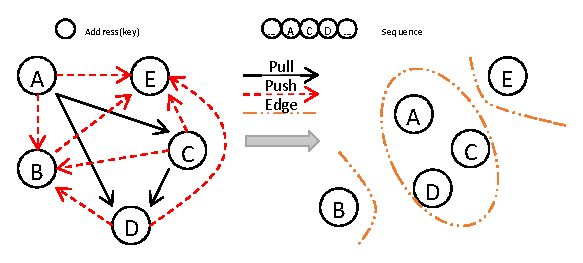
\includegraphics[width=0.9\linewidth]{fig/sequence_grouping.eps}
\caption{Temporal-aware Sequence Classification.}
\label{fig:sequence_grouping}
\end{figure}

\subsection{Graph-based I/O Classification}

To address the issues of the statistical-based approach, as shown in Figure~\ref{fig:sequence_grouping},
we propose graph-based approach which procedure is similar but essentially different.
Instead of binding the addresses with a probability matrix,
As shown in Figure~\ref{fig:sequence_grouping}, we adopt a graph-based approach which
maps the addresses to points in a $N$-dimensional linear space.
Upon the arrival of the requests, the points of correlated cells apply attractive force to each other while the uncorrelated ones apply repulsive force.
As the points moving in the space, they will gradually form clusters while those clusters will be separated by repulsion.
In this process, the repulsive force serves as regularization and makes the points more equally distributed.
For example, if address A, C and D appeared together in the sequence sliding window,
the algorithm will pull them closer in the N-dimensional space,
so that the classification algorithm can categorizes them into one class.
On the convergence of the movement, clustering algorithms are adopted to assign the points into groups.
With the combination of the physical movement and clustering, this approach obtains a better division as well as being robust to noise.

\begin{equation}
\label{eq:physicalbasedequation}
feature_{dst} = (1 - \lambda) \cdot feature_{dst} + \lambda \cdot mean(feature_{src})
\end{equation}

Moreover, in some cases, highly correlated addresses share a close accessing frequency.
An additional term is introduced to reflex this consideration by applying extra movement based on their access frequency.
And a frequency factor is involved to lever the weight of this term, which is adjustable for specific file systems and applications.
The equation for this term is in Equation~\ref{eq:frequencyterm}:

\begin{equation}
\label{eq:frequencyterm}
feature = (1 - \epsilon) \cdot feature + \epsilon \cdot frequency
\end{equation}
in which $\epsilon$ represents the frequency factor.
% And the complete procedure of TAC is presented in Algorithm~\ref{tacphysical}.

In real-world scenario, the number of concurrent threads is varying over time.
The graph-based approach maps the addresses based on their correlation rather than setting hard boundaries on division,
which makes it possess the potential to solve this issue.
% We leave this exploration to future work.

\iffalse
\begin{algorithm}
\caption{The procedure of TAC algorithm}
\label{tacphysical}
\begin{flushleft}
\textbf{Input:} $trace$, $ng$(number of groups), $interval$, $criterion$, $\lambda$(updating factor), $\epsilon$(frequency factor)
\linebreak
\textbf{Output:} $mp$(mapping table)
\end{flushleft}
\begin{algorithmic}[1]
  \State $na \gets$ \#addresses appeared in trace
  \State $freq \gets$ normalized frequency of addresses appearance
  \State $table \gets$ random matrix of $na \times ng$
  \State $table \gets \textbf{Standardize}(table)$
  \State $step \gets criterion + 1$
  \While{$step > criterion$}
    \State $target \gets$ \textbf{Target}($trace,na,ng$)
    \State $step \gets \textbf{mean}(target-table)$
    \State $table \gets (1-\lambda) \cdot table + \lambda \cdot target$ \Comment apply attractive force
    \State $table \gets (1-\epsilon) \cdot table + \epsilon \cdot freq$ \Comment extra movement regularized by frequency
    \State $table \gets \textbf{Standardize}(table)$ \Comment{expansion as repulsion}
  \EndWhile
  \State $mp \gets \textbf{Clustering}(table)$
  \State \textbf{return} $mp$
\end{algorithmic}
\hspace{0.6cm}- - - - - - - - - - - - - - - - - - - - - - - - - - - - - - - -
\begin{algorithmic}[1]
  \Function{Standardize}{$table$}
    \State $\mu \gets$ mean $w.r.t.$ rows of $table$
    \State $\sigma \gets$ deviation $w.r.t.$ rows of $table$
    \State $table \gets (table - \mu) / \sigma$
    \State \textbf{return} $table$
  \EndFunction
\end{algorithmic}
\hspace{0.6cm}- - - - - - - - - - - - - - - - - - - - - - - - - - - - - - - -
\begin{algorithmic}[1]
  \Function{Target}{$trace,na,ng$}
    \State $target \gets$ zero matrix of $na \times ng$
    \For{$dst$ in $trace$}
      \State $src \gets$ addresses appeared within
      \State \hspace{1.05cm}$interval$ before $dst$ in $trace$
      \State $target(dst) \gets target(dst)+mean(table(src))$
    \EndFor
    \State \textbf{return} $target$
  \EndFunction
\end{algorithmic}
\end{algorithm}
\fi

\iffalse
\begin{figure}[h]
\centering
\includegraphics[width=0.9\linewidth]{fig/multi_scale_grouping.eps}
\caption{Illustration of Multi-scale Workload Identification.}
\label{fig:multi_scale_grouping}
\end{figure}

\subsubsection*{Step 2: Multi-scale Workload Classification}

It is common to physically isolate the data from different applications both
for the performance and security purpose~\cite{huang2017flashblox}.
This ispire us to do multi-scale classification.
To achieve this, we need to submit the application's information together with the I/O requests to the low level disks,
which needs a large investment of changes in the storage subsystem.
It is more challenge when virtualization technique are deployed.
For example, system managers would use different filesystem configurations
for different applications.
However, if the managed system runs in a virtualized environment,
it would be more challenge to config properly.
Another solution is to estimate the necessary information
based on the learned I/O patterns,
so that we can develop an automatic performance tuning technique.
This lays in the fact that different application
will generate significantly different I/O pattern.
We can use a sequence classification technique to identify the workloads,
and then enable different workload-aware optimization methods.
Not only the application I/O, we may also identify the system workloads,
such as distinguish the filesystem from the I/O pattern.
To solve this, we propose to do multi-scale workload classification as shown in Figure~\ref{fig:multi_scale_grouping}.
In the first layer, we do cross-grained classification to distinguish different types of workloads.
As a result, substantially different workloads can be isolated.
Then in the second layer, we can further apply our temporal-aware classification
to study fine-grained request relationships.
\fi

\section{Evaluation}

% We employ our open-sourced SSD emulator~\cite{zhou2018cpftl} to implement
% a prototype system of learned log-structured storage architecture.
To develop a working system within a reasonable time frame,
most of existing ML frameworks expose their programming interfaces through
high-level programming languages, such as Python and Java.
This also allows for ease of tuning of ML algorithms and execution parameters.
However, current main stream storage systems are developed in C/C++.
A great portion of them runs at kernel device driver level or even device firmware level.
It is an intimidating job of developing ML algorithms at either device driver or firmware level.
More importantly, it could be infeasible to conduct sensitivity
test and tune different ML algorithms at low level architectures.

Our idea is to develop a working system on top of our open-sourced SSD emulator~\cite{zhou2018cpftl},
which reserves a large physical DRAM space to mimic the external storage devices. Our in-house GPU cluster serves as the host, among which node is configured with 2 Intel Xeon E5, 2.2 GHz 12-core, 128GB and four NVIDA GeForce GTZ Titan XP Graphics card, 12 GB GDDR5X cards. 
We offload most of the low-level functionalities
at either kernel space or device firmware to the user space.
In the user space, we are free to choose any high-level ML libraries
and programming languages for quick implementation.
Once the prototype system is tuned well and validated mature,
we can move forward to re-implement the functions by the low-level languages.

Figure~\ref{fig:emulator_architecture} shows the architecture of SSD emulator
based learned storage prototype.
At kernel space, SSD emulator reserves large amounts of contiguous memory
at boot time as the emulated flash memory.
The NVMe protocol with 65K queues is built to directly handle the logic page number of logic block request (LBA in brief).
Since current library support at kernel space is very limited,
we implement Flash Translation Layer (i.e., FTL in brief) at user space.
For efficiency, we employ a validated version of our in-house correlation-aware FTL
protocol to perform address translation between logical page number and physical page number.
It adopts bloom filter~\cite{gremillion1982designing} algorithm find the correlations among the LBA requests and define the corresponding mappings.

\subsection*{Preliminary Results}

To gauge the effectiveness and efficiency of our proposed learned log-structured storage architecture,
we conducted a comprehensive set of experiments, and collected preliminary results about the cache hit ratio of I/O accesses
for our working SSD Emulator based prototype.
We implemented the FTL module using different cache and prefetching algorithms.
Regarding the learned I/O prefetcher module,
we first implemented our temporal-aware classification (TAC) algorithm to split mixed workloads.
Afterwards, we employ the LSTM model to predict the future I/Os.
We used both synthetic and real-world traces and divided traces into training part and testing part.

\begin{figure}[t]
  \centering
  \begin{subfigure}[b]{0.45\textwidth}
    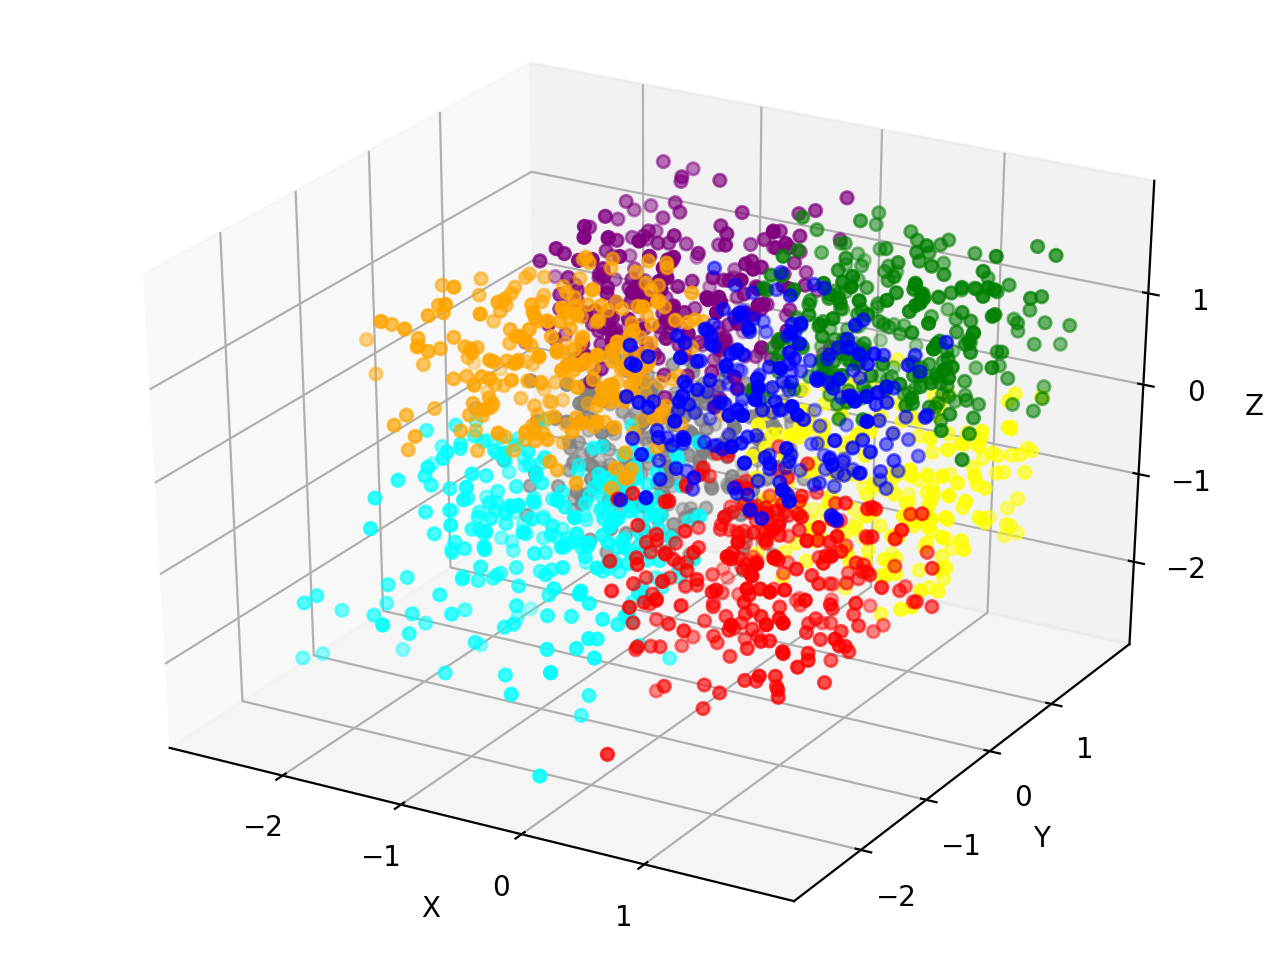
\includegraphics[width=\textwidth]{fig/fig_step_10_2000.png}
    \caption{8 files classification.}
    \label{fig:8files}
  \end{subfigure}
  \begin{subfigure}[b]{0.45\textwidth}
    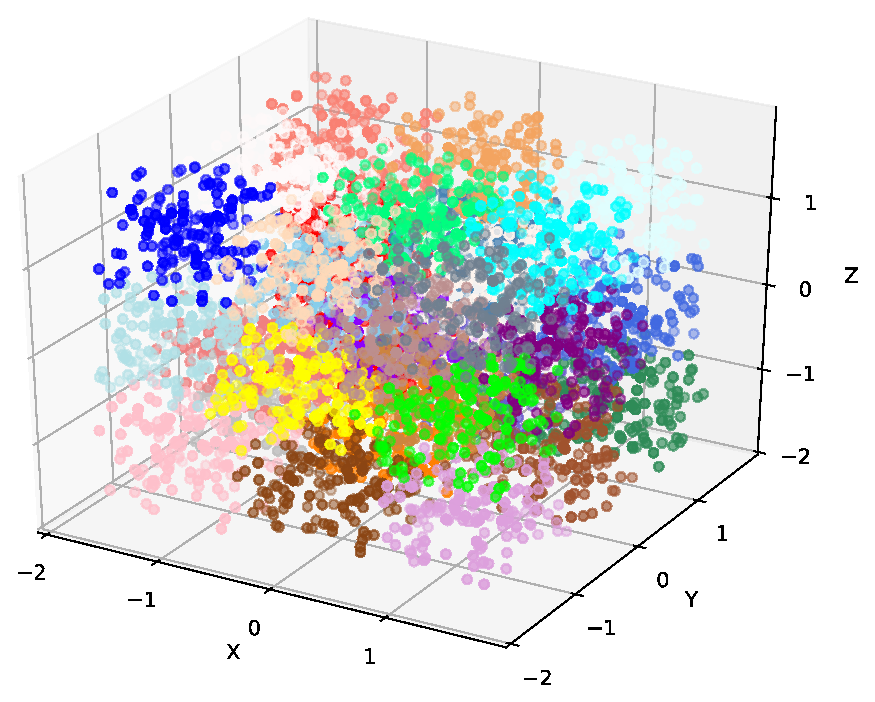
\includegraphics[width=0.85\textwidth]{fig/fig_step_32_6_150.eps}
    \caption{32 files classification.}
    \label{fig:32files}
  \end{subfigure}
  \caption{Temporal-aware sequence classification. The addresses are mapped into dots at a 3-dimensional linear space. Addresses from different files are distinguished by color.}
  \label{fig:files}
\end{figure}

In Figure~\ref{fig:files}, we demonstrate the effectiveness of our TAC algorithm in classifying the entangled I/O workloads.
We collect the I/O trace under a dedicated multi-thread workload.
We then label all I/O request with the corresponding file id.
TAC is an unsupervised classification algorithm that classify the I/O address
in a way that the address belonging to one file is in the same cluster and vice versa.
Without loss of generality, we only show 8 files and 32 files classification in 3-dimensional linear space respectively.
However, when the number of files grows, the classification results will follow the same principles.
Obviously, as the attractive and repulsive force move the dots, the addresses from the same file gradually form clusters,
and addresses from different files are effectively separated.

\begin{figure}
\centering
\begin{minipage}{.45\textwidth}
  \centering
  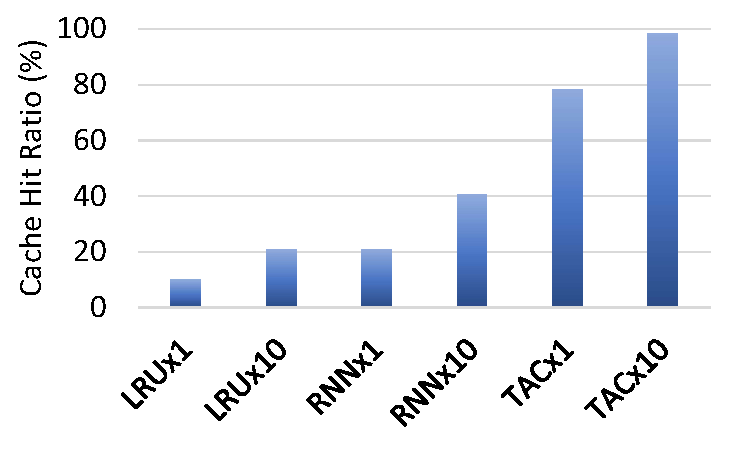
\includegraphics[width=0.8\textwidth]{fig/cache.eps}
  \caption{Average cache hit ratio.}
  \label{fig:cache}
\end{minipage}
\begin{minipage}{.45\textwidth}
  \centering
  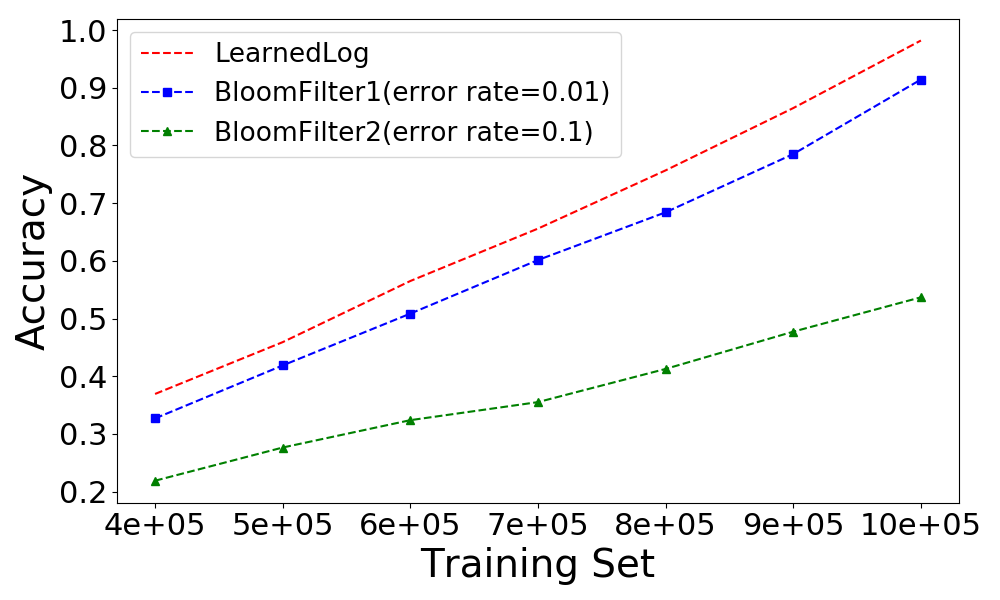
\includegraphics[width=0.8\textwidth]{fig/log2.png}
  \caption{Predicting accuracy of Learned Log.}
  \label{fig:learned_log}
\end{minipage}%
\end{figure}

By using the TAC, we split the workloads into multiple clean I/O streams.
We then use the RNN model to predict the future I/Os.
We split the collected I/O trace into training and testing datasets.
We use the trained models to do the I/O prefetch and study the cache hit ratio,
and compare the performance of the traditional LRU cache,
the default LSTM (RNN) prefetcher, and the TAC + LSTM (TAC) prefetcher.
Figure~\ref{fig:cache} shows the cache hit ratio using different configurations.
We use $10^4$ files and use $0.1\%$ (in x1) and $1\%$ (in x10) respectively.
RNNx1 prefetch the first candidate predicted by the RNN model.
RNNx10 prefetch the top 10 candidates predicted by the RNN model.
TAC is the RNN with temporal-aware classification sitting in front.
TACx1 prefetch the first candidate of the RNN prefetcher.
TACx10 prefetch the top 10 candidates of the RNN prefetcher.
LRUx1 use LRU cache and reserves the same amount of cache space as the RNNx1.
LRUx10 use LRU cache and reserves the same amount of cache space as the RNNx10.
Given new learned I/O prefetcher,
we improve the cache hit ratio by 5-6 times for modern storage architecture.

Figure~\ref{fig:learned_log} shows the prediction accuracy of our learned log.
Given enough training data, our learned log can achieve up to $99\%$ accuracy
in predicting the last occurring position of a key in the log.
Comparing to the bloom filter, which achieves a very close level of accuracy, learned log save 70\% of memory.

% In summary, our preliminary work showed very promising results.
% Equipped with new learned log-structured storage module, we save 70\% of memory space?
% In terms of log management related in-memory data structures without compromising performance.

\input{conclusion}

\bibliographystyle{ieeetr}
\bibliography{out/auto-merge}
\end{document}
